\section{Summary of the studies}
Using field sampling and laboratory infection of wild and wild-derived mice from the European house mouse hybrid zone (HMHZ) between \textit{M. m. domesticus} and \textit{M. m. musculus}, we asked (1) whether hybrid mice are more or less resistant than their parents to \textit{Eimeria} spp., and (2) whether resistance and tolerance are decoupled in two \textit{Eimeria} species. \par

In \textbf{Chapter 2}, we found that for both intracellular \textit{Eimeria} spp. and extracellular pinworms, parasite intensities are significantly lower in hybrid mice than in parental genotypes. We tested potential over or under-mortality of hybrids, as well as difference of prevalence in the centre of the zone, and could not detect either of these effects. We concluded that hybrid mice are more resistant to parasites than their parents in this system (\textbf{Figure 4.1}).

\begin{figure}[H]
    \centering
    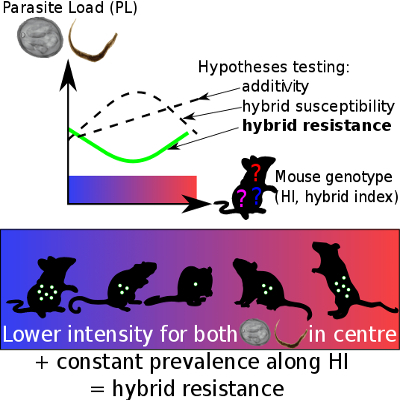
\includegraphics[width=.5\linewidth,height=\textheight,keepaspectratio]{images/4discussion/Figure3.jpg}
    \caption{\textbf{Lower intensity of infection with intracellular \textit{Eimeria}~spp. and extracellular pinworms in the centre than in the edges of the HMHZ without evidence of decreased parasite prevalence towards the centre: hybrid resistance hypothesis is favoured}. The hybrid index is represented as a gradient ranging from 0 (pure Mmd, in blue) to 1 (pure Mmm, in red)}
\end{figure}

\par
These findings alone do not allow to draw conclusions on hybrid host fitness in relation to parasites. In order to do so, there is a need to investigate the link between resistance and host health, or more precisely to test the coupling between resistance and tolerance, which was the second aim of this thesis. In \textbf{Chapter 3}, we infected four wild-derived inbred strains, two Mmd and two Mmm, with three isolates from two \textit{Eimeria} species, namely \textit{E.~falciformis} and \textit{E.~ferrisi}. We found a trade-off between resistance and tolerance for \textit{E.~falciformis}, and that these defense mechanisms were decoupled for \textit{E.~ferrisi}. We demonstrated the necessity of studying not only resistance but also tolerance in order to assess the impact of parasite on health, and to do so at the parasite species level (\textbf{Figure 4.2}). 

\begin{figure}[H]
	\centering
	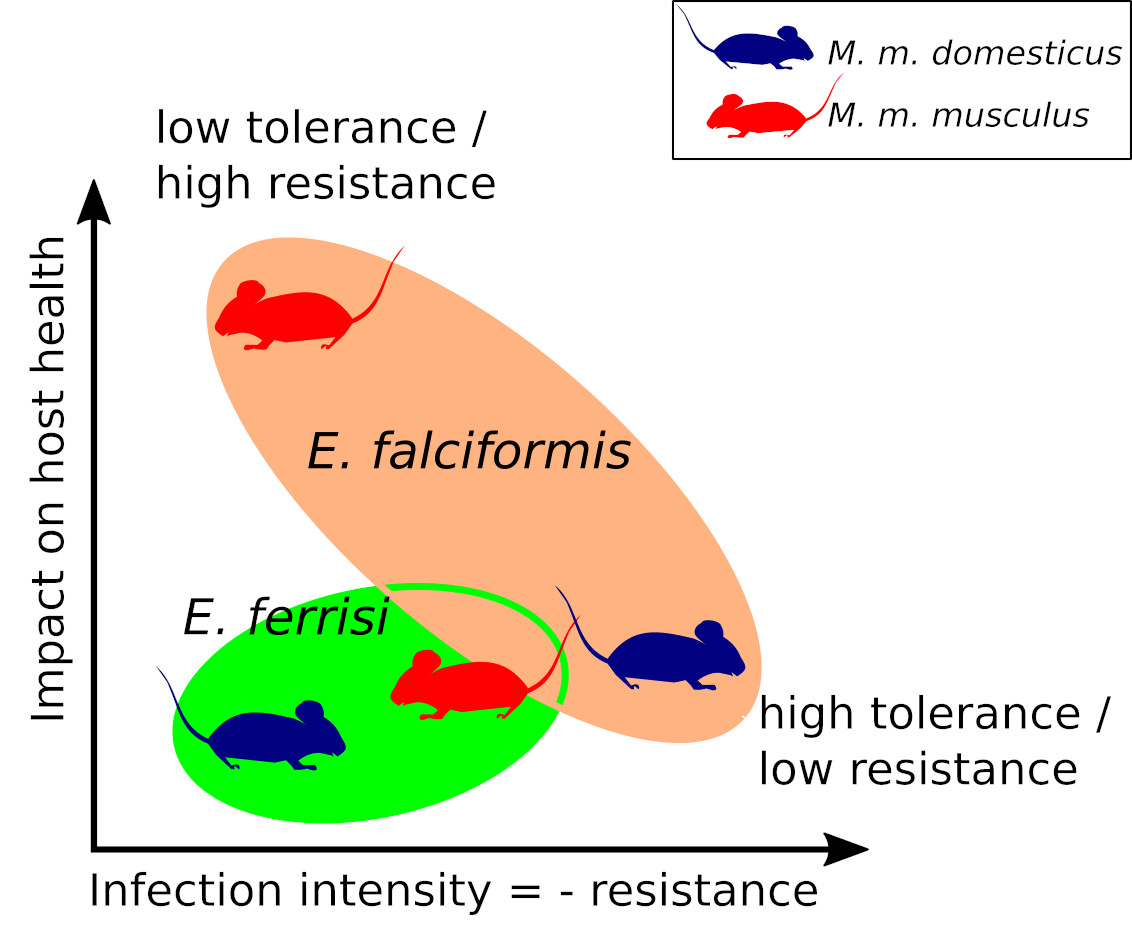
\includegraphics[width=.5\linewidth,height=\textheight,keepaspectratio]{images/4discussion/Figure4.jpeg}
	\caption{\textbf{Coupling between resistance and tolerance for two different \textit{Eimeria} species}. Upper left corner: low tolerance area (strong impact on health despite low parasite load). Lower right corner: high tolerance area. We found a resistance/tolerance trade-off upon infection with \textit{E.~falciformis}, absent in the case of \textit{E.~ferrisi}}
\end{figure}

The results of our first study (\textbf{Chapter 2}) indicate that hybrid mice resist parasites better than parental subspecies. If there are incompatibilities in the hybrid genomes associated with resistance, they are likely compensated by the advantage of recombinations. As presented in the introduction of this thesis, previous field studies and laboratory experiments failed to reach a consensus. We believe it is necessary to review previous studies on hybrid resistance in this system in an attempt to settle the debate.

\section{Discrepancies between studies on hybrid resistance or susceptibility to parasites in the HMHZ are likely explained by methodological issues}
At the light of our new results, and in order to understand the discrepancies between studies, we summarise in \textbf{Table 4.1} the key characteristics of each study explicitly addressing differences between hybrid and parental subspecies parasite load in the HMHZ. \par
Reviewing the main differences between all studies, we see first that there seems to be a change over time, from hybrid susceptibility to hybrid resistance. In particular, the two field studies concluding on hybrid susceptibility \citep{sage_wormy_1986, moulia_wormy_1991} rely on data collected about twenty years earlier than the two field studies concluding on hybrid resistance \citep{baird_where_2012, Balard2020}. One could suspect a change of hybrid response to parasite in terms of resistance of susceptibility over time. Indeed, \cite{wolinska_parasites_2008} proposed that parasites could represent a dynamic selective force in hybrid zones. Frequency-dependent selection could explain oscillations between hybrid resistance and hybrid susceptibility scenarios. According to this model, parasites adapt alternatively to the most common host taxon, represented either by parents or by hybrids. If parasites decrease host fitness, the relatively more infected host taxon decreases in prevalence. Eventually the other taxon becomes the most common one, targeted by parasites, and the cycle goes on. Nevertheless, as noted by \cite{baird_where_2012}, the HMHZ system lacks F1 and early generations hybrids: late generation, highly recombinant hybrids represent a highly diverse genetic pool of individuals rather than one homogeneous taxon. Thus, this frequency-dependent selection dynamic is unlikely to apply in our system. Then, the question of hybrid resistance/susceptibility has been asked in a full range of geographical locations (column “Origin of mice” of \textbf{Table 4.1}). Hybrids could be either more susceptible or resistant to parasites in different part of the zone. This is nevertheless contradicted by the fact that several studies performed in Germany on the same parasites, intestinal helminths, showed opposite results \parencites[hybrid susceptibility for][hybrid resistance for]{sage_wormy_1986}{baird_where_2012, Balard2020}. 

\begin{table}[H]
	\centering
	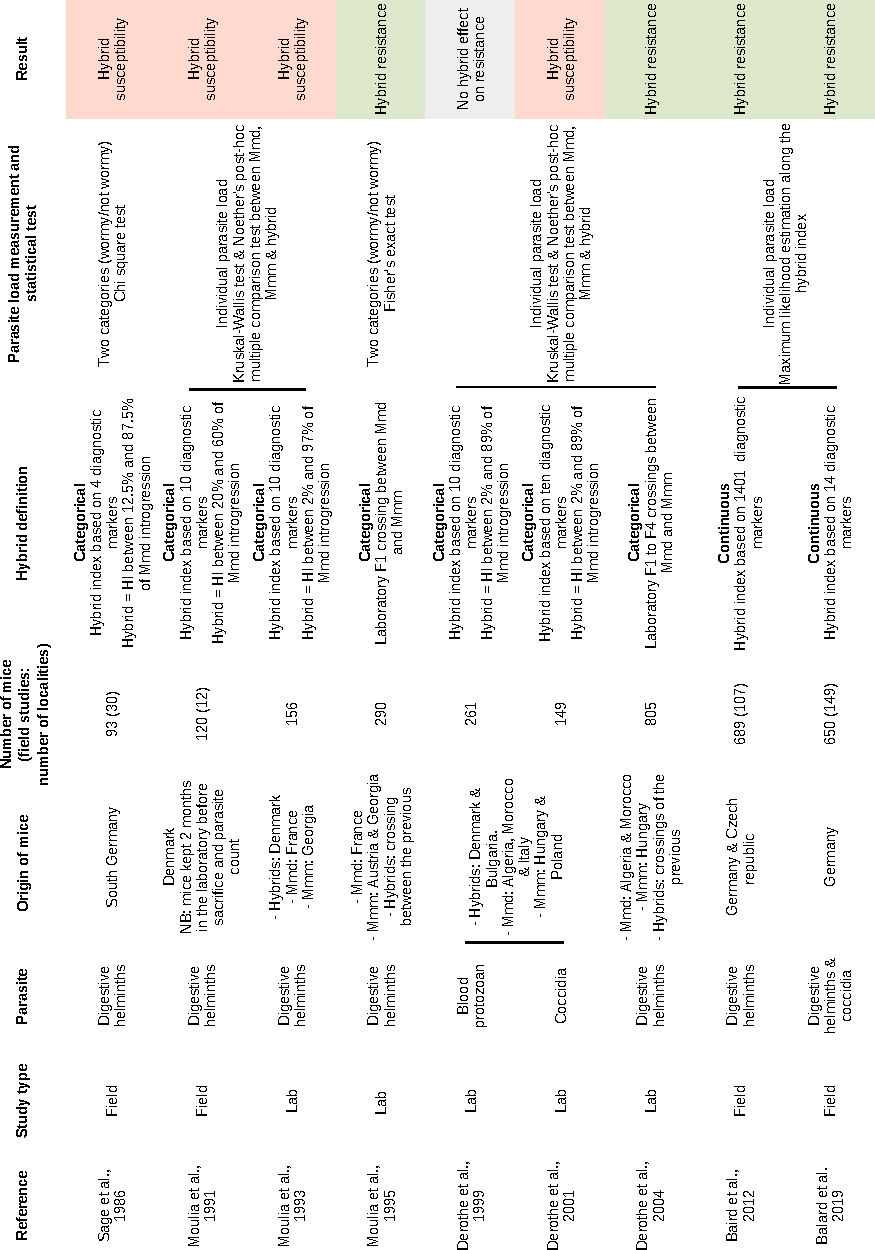
\includegraphics[width=\linewidth,height=\textheight,keepaspectratio]{images/4discussion/Table1.pdf}
	\caption{\textbf{List of studies addressing relative parasite load of hybrids compared to parental subspecies in the HMHZ}. The last column shows the main result of each study, either “hybrid susceptibilities” if hybrids were found to harbour significantly more parasites than parental subspecies, “hybrid resistance” in the opposite case, and in one case “no hybrid effect on resistance” if no significant difference between parasite load in hybrids and parental subspecies could be detected.}
\end{table}

Technical and statistical differences between the studies seem more likely to explain the observed discrepancies. One major difference between studies is the characterisation of hybrids (see \textbf{Table 4.1}). The two more recent studies (including ours), besides examining the highest number of mice, considered these mice on a continuum of hybridization rather than as in arbitrary categories. Moreover, each study using the categorical approach used a different threshold, the more stringent \cite{moulia_wormy_1991} considering that a mouse presenting between 20 to 60\% of Mmd alleles constitutes a hybrid, the more relaxed (\cite{moulia_experimental_1993}) 2 to 97\%. Dichotomization of continuous variables, the practice of converting data sampled along a continuum into categories, is harmful to data analysis \citep{maccallum_practice_2002}. In our system, if there is an effect of hybridization on immune genes, hybrid resistance or susceptibility must be higher in the most introgressed mice \citep{baird_where_2012}. Dichotomization of hybrid index ignores this relationship, and can mislead the results. 
\par
To conclude on this section, we can say that the pioneer study \cite{sage_wormy_1986} raised a fascinating question regarding the possible role of parasites in the hybridization process. About this first work, \cite{klein_book_1988} wrote that “the data are too preliminary to qualify for inclusion in a textbook”. He qualifies the conclusion of this study “a finding that still awaits confirmation on a truly representative sample”. It seem likely that original limitations of statistical methods are the main reason for the observed discrepancies in the follow up works. At the light of our summarized review, we can be confident that hybrids in the HMHZ are more resistant to parasites than parental subspecies.
\par
As described in the introduction of this thesis, there has been a long lasting controversy on (1) the relative load of parasites in hybrids vs. parentals, and (2) the effect of parasitism as selective factor against hybrid mice in the HMHZ. Once agreed on the direction of hybrid effect on resistance to parasite, one needs to question the actual effect of an increased resistance on the overall fitness of hybrids.

\section{Studies of parasite selective pressure on their hosts require a switch of focus from resistance to tolerance}
Since the end of 1990s, numerous studies have discussed the role of parasites in hybridizing animal systems (see reviews by \cite{fritz_resistance_1999}, \cite{karvonen_role_2012} and \cite{theodosopoulos_parasites_2019}). Of note, \cite{baird_shifting_2019} argue that directly linking differential resistance to differential fitness in hybrids compared to parents is a dangerous shortcut, because tolerance could distort the link between parasite load and fitness. Unfortunately, only a few studies focusing on parasite as selective factors in hybridizing systems measure jointly resistance and tolerance in hybrids compared to parents. For example, in the freshwater snails genus \textit{Melanopsis}, resistance against trematodes was found higher in hybrids than in parental taxa, and damaging parasite-induced gigantism (a measure of tolerance) was absent in hybrids and present in all parental taxa \citep{guttel_maintenance_2014}. Such approach truly allows to conclude on an impact of parasitism on the maintenance of species barrier in this system. 
\par
In our system, the field study alone allowed to test relative hybrid resistance, but testing relative hybrid tolerance was particularly challenging (\textbf{Chapter 2}). Moreover it would not have been possible to test the difference between \textit{Eimeria} species in the field due to the low prevalence of \textit{E.~falciformis} leading to a lack of statistical power. We chose to use a complementary laboratory approach to address resistance and tolerance altogether. Although laboratory inbred mice represent only a small proportion of the diversity observed in the wild, we were able to gain insight on the coupling of resistance and tolerance in both parental subspecies (\textbf{Chapter 3}). More specifically, Eastern mice (Mmm) strains resist the parasite \textit{E.~falciformis} similarly or even more than Western (Mmd) mouse strains, but do not tolerate it as well. We can argue that the tolerance mechanisms involved in response to infection by this parasite differ in each host subspecies. During hybridization, the increased resistance of hybrids against \textit{Eimeria} likely comes from recombinations in parts of the immune system responsible of resistance (\textbf{Chapter 2}). There is no evidence that tolerance, especially if implying different mechanisms in each parental subspecies, would be affected the same way upon hybridization. Preliminary experimental infection of four F1 crossings (two outbred pure subspecies (Mmd or Mmm), and two Mmd-Mmm hybrids) did not allow to detect effect of hybridization on tolerance (unpublished data), though this experiment contained a low number of mice and has to be repeated to gain sufficient statistical power. At this stage, we might still assume that parasites could play a role as selective factor advantaging (or penalising) hybrids in the HMHZ, even if our sample does not show such a role, which is an incentive for further experimental testing.

\section{Conclusion and perspective}

During this PhD project, we argue that we settled the debate on hybrid resistance or susceptibility to parasites in the European house mouse hybrid zone: hybrid mice are more resistant to parasites than parental host subspecies, and contradicting results of part of the previous studies likely find their origin in technical and statistical limitations. Moreover, we found differences in coupling of resistance and tolerance between two closely related parasites in laboratory infection, showing the necessity of measuring jointly resistance and tolerance before drawing conclusions on the impact of parasitism on species barriers. \par

In future, relative tolerance in hybrids compared to parental mice could be assessed in a control setting. To control for the deleterious effects of inbreeding, one should compare tolerance to both \textit{Eimeria} species between intra- and inter-subspecies mouse groups, using for example the maximum likelihood optimization approach developped in \textbf{Chapter 2}. This would allow to finally tackle the issue of impact of parasite on species barrier in this system.
